\documentclass[11pt, a4paper]{article}
\usepackage[utf8]{inputenc}

\usepackage[margin=1in]{geometry} 
\usepackage{amsmath,amsthm,amssymb}
\usepackage[margin=1in]{geometry} 
\usepackage{amsmath,amsthm,amssymb}

\usepackage[slovene]{babel}
\usepackage{color}
\usepackage{graphicx}
\usepackage{amssymb}
\usepackage{amsmath}
\usepackage{mathtools}
\usepackage{commath}
\usepackage{ragged2e}
\usepackage[T1]{fontenc}
\usepackage[normalem]{ulem}
\usepackage{amsthm}
\usepackage{esvect}
\usepackage{float}
\usepackage{calrsfs}
\DeclareMathAlphabet{\pazocal}{OMS}{zplm}{m}{n}
\newcommand{\Ga}{\mathcal{G}}
\mathtoolsset{showonlyrefs} 

\newcommand\setItemnumber[1]{\setcounter{enumi}{\numexpr#1-1\relax}}


\newtheorem{theorem}{Trditev}[section]
\newtheorem{corollary}{Posledica}[section]
\newtheorem{lemma}[section]{Lema}
\theoremstyle{definition}
\newtheorem{definition}{Definicija}[section]
\theoremstyle{example}
\newtheorem{example}[section]{Primer}
\theoremstyle{izrek}
\newtheorem{izrek}[section]{Izrek}

\begin{document}
\begin{center}
\thispagestyle{empty}
\parskip=14pt%
\vspace*{3\parskip}%
\begin{Huge} Določanje Boltzmanove konstate \end{Huge}

By

Matic Tonin

ID No. (28181098)

Mentor 

(Rok Dolenec)

\rule{7cm}{0.4pt}

Pod okvirom:

FAKULTETE ZA FIZIKO IN MATEMATIKO, LJUBLJANA

1. 4. 2020

\end{center}
\pagebreak
\section{Naloga}
\begin{enumerate}
\item Umerite kotno skalo spektroskopa s spektralnimi crtami Hg in $H_2$.
\item Izmerite valovne dolžine spektralnih crt v spektru varcne žarnice. Primerjajte spekter
s tistim, izmerjenim v Hg pod tocko 1.
\item Izmerite centralno valovno dolžino in ocenite spektralno širino rdece, rumene, zelene
in modre svetlece diode (LED).
\item Opazujte zvezni spekter volframove žarnice in oceni valovno dolžino najsvetlejšega
(rumenega) dela in zapišite intervale, ki jih pokrivajo posamezne barve.
\item  Opazujte absorpcijski spekter $NO_2$ tako, da cevko s plinom presevate z belo svetlobo.
\item Izmerite valovne dolžine crt v spektru He in Ne.
\end{enumerate}
\section{Potek dela}
Najprej postavimo postavitev, kot nam jo prikazuje slika v navodilih:
\begin{figure}[H]
    \centering
    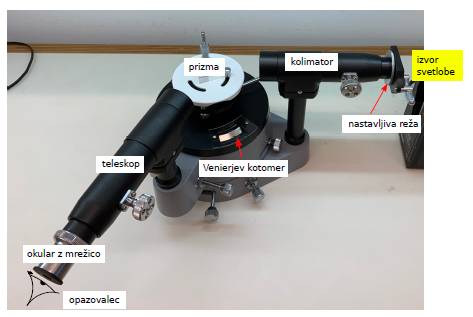
\includegraphics[width=10cm]{Postavitev.png}
    \caption{Prikaz postavitve meritve}
\end{figure}
Za vsako meritev bomo merili kot čim bolj natančno, torej vsaj do minute natančno, zato bomo uporabljali Vernierovo skalo. Princip je podoben kot kljunasto merilom. Najprej pa moramo kotomer umeriti, zato opazujemo spektre z že poznanimi valovnimi dolžinami. Pri meritvah moramo vedno opazovati tisti rob reže, ki je fiksen. Emisijske spektre plinov opazujemo lahko le, ko je plin ioniziran. Zato ga priklopimo na izvor napetosti in pri tem pazimo, da je preden damo vanj kapsulo s plinom, ugasnjen. Ampule na nosilcu se med meritvijo ne dotikamo. 
Izmerimo šže znane črte za Hg in $H_2$, za katere bomo nato s fitano funkcijo vedeli kakšne so kalibracijske konstante za ostale svetlobe. Po opravljeni kalibraciji si ogledamo še emisijske spektre svedlobe iz LED diod, varčne žarnice in volframove žarnice. Za $NO_2$ pa pred volframovo žarnico postavimo ampulo in si zabeležimo vidne črte.

\section{Meritve}
\subsection{Kalibracija kotomera}
\subsubsection{Emisijski spektri Hg}
Iz teorije vemo, da plini sevajo črtaste spektre določenih valovnih dolžin. Te so določeni z energijo elektronskih prehodov v atomih plina in za Hg so značilne naslednje črte. Če zraven, zaradi zbranosti podatkov navedemo še izmerjene kote, dobimo tabelo:
\begin{table}[H]
	\centering
	\begin{tabular}{|c|c|c|}
		\hline
		Barva &  $\lambda$ [nm] & Izmerjen kot [°] \\
		\hline
		\hline
		Rumena  & 577 & 174°20'\\
		\hline
		Rumena  & 597 & 174°15'\\
		\hline
		Zelena & 546 & 173°35'\\
		\hline
		Modrovijolična & 436 & 169°25' \\  
		\hline
		\hline
	\end{tabular}
	\caption{Podatki o znanih valovnih dolžinah spektralnih črt Hg}	
\end{table}
Na žalost nismo uspeli videti tudi vijolične črte, ki bi jo našli pri 405 nm. Razlog za to je, da je oko manj občutljivo za vijolični spekter in je zato od posameznika odvisno, ali vidi ta del spektra ali ne. \\
\medskip
Če narišemo umeritveno krivuljo za Hg spekter, da vemo kolikšne so konstante za naš kotometer in prizmo. Fit naše funkcije se glasi:

$$kot=c_1+c_2\lambda+c_3 \sqrt{\lambda}$$

Če si sedaj narišemo to funkcijo za Hg, dobimo:

\begin{figure}[H]
    \centering
    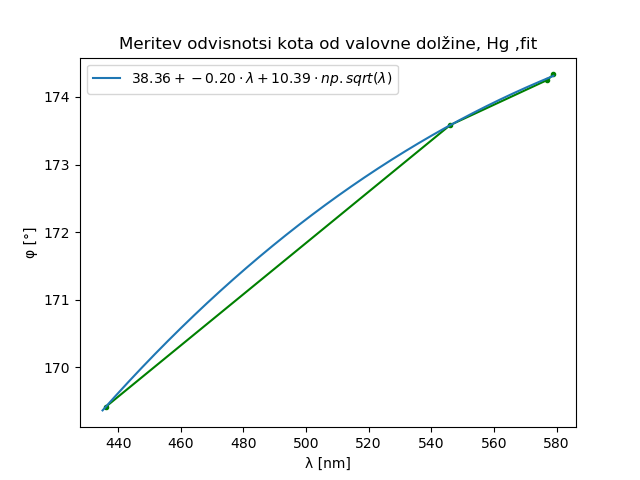
\includegraphics[width=12cm]{Hg spekter,fit.png}
    \caption{Prikaz meritev za Hg celico}
\end{figure}
Za katero je funkcija kar enaka legendi grafa.
\subsubsection{Emisijski spekter $H_2$}
Če prav tako za $H_2$ naredimo tabelo znanih vrednosti dobimo:
\begin{table}[H]
	\centering
	\begin{tabular}{|c|c|c|}
		\hline
		Barva &  $\lambda$ [nm] & Izmerjen kot [°] \\
		\hline
		\hline
		Rdeča  & 656 & 175°50' \\
		\hline
		Svetlomodra  & 486 & 171°45'\\
		\hline
		Modrovijolična & 434 & 169°25'\\
		\hline
		Vijolična & 410 & // \\  
		\hline
		\hline
	\end{tabular}
	\caption{Podatki o znanih valovnih dolžinah spektralnih črt $H_2$}	
\end{table}
Če tudi za ta del vaje narišemo graf, dobimo:
\begin{figure}[H]
    \centering
    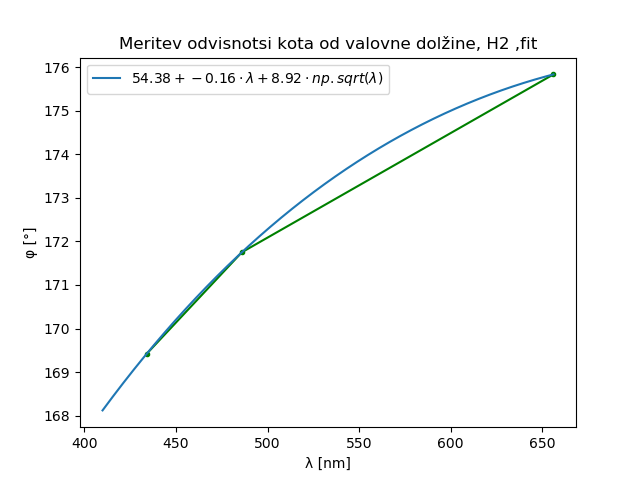
\includegraphics[width=12cm]{H2 spekter,fit.png}
    \caption{Prikaz meritev za $H_2$ celico}
\end{figure}
\subsubsection{Skupni spekter}
Zaradi določanja konstant na funkciji:
$$kot=c_1+c_2\lambda+c_3 \sqrt{\lambda}$$
narišemo oba spektra hkrati in skozi potegnemo graf. S tem bomo določili konstante $c_1, c_2, c_3$, ki so konstante naše priprave. S tem bomo kasneje lahko določali valovne dolžine naših svetil.
Graf se glasi:
 \begin{figure}[H]
    \centering
    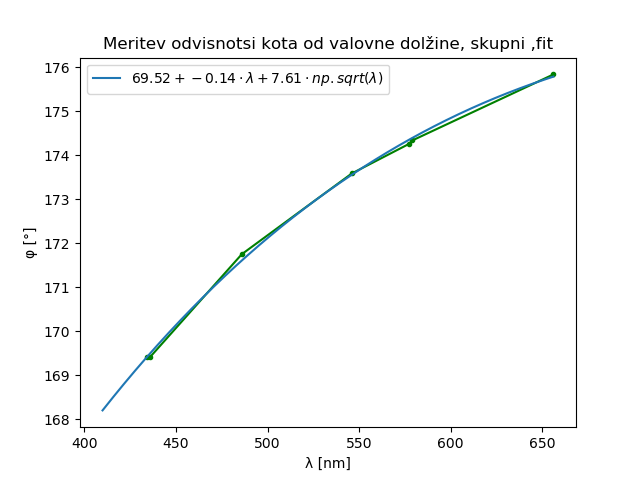
\includegraphics[width=12cm]{Skupni spekter,fit.png}
    \caption{Prikaz skupnih meritev za določanje konstant}
\end{figure}

Tako vemo da je naša funkcija za določanje valovnih dolžin enaka:
$$kot=69.5616-0.135 \cdot \lambda+7.6056\cdot \sqrt{\lambda}$$
\pagebreak
\subsection{Merjenje valovnih dolžin svetil}
\subsubsection{Varčna žarnica}
Da bi izmerili črtasti spekter varčne žarnice, moramo najprej zapisati formulo za izračun valovne dolžine. To dobimo z obračanjem enačbe, ki smo jo določili pri prejšnjem poglavju. Dobimo, da je:

$$\lambda=\left(\frac{-7.61 \pm\sqrt{7.61^2+4 \cdot 0.14(69.52-\phi)}}{-2 \cdot 0.14}\right)^2$$
kjer je kot podan v stopinjah.

Če podamo tabelo, kjer bomo računali vrednosti za vsak kot posebej, dobimo:
\begin{table}[H]
	\centering
	\begin{tabular}{|c|c|c|}
		\hline
		Barva &  $\lambda$ [nm] & Izmerjen kot [°] \\
		\hline
		\hline
		Vijolična  & 434 & 169°25' \\
		\hline
		Modrozelena  & 485 & 171°35' \\
		\hline
		Zelena & 549.5 & 173°40'\\
		\hline
		Rumena & 575.88& 174°20'\\  
		\hline
		Rumena & 579.46 & 174°25'\\  
		\hline
		Rdeča & 625.4 & 175°20' \\  
		\hline
		\hline
	\end{tabular}
	\caption{Podatki o varčni žarnici}	
\end{table}
\subsubsection{Volfram žarnica}
Spet uporabimo formulo:
$$\lambda=\left(\frac{-7.61 \pm\sqrt{7.61^2+4 \cdot 0.14(69.52-\phi)}}{-2 \cdot 0.14}\right)^2$$
kjer je kot podan v stopinjah.

Če podamo tabelo, kjer bomo računali vrednosti za vsak kot posebej, dobimo:
\begin{table}[H]
	\centering
	\begin{tabular}{|c|c|c|c|c|}
		\hline
		Barva &  $\lambda_1$ [nm]&  $\lambda_2$ [nm] & Izmerjen kot 1 [°] & Izmerjen kot 2 [°]\\
		\hline
		\hline
		Vijolična  & 396.9 & 454& 167°30'	&170°20' \\
		\hline
		Modra  & 454.2 & 487.2& 170°20'& 171°40' \\
		\hline
		Zelena & 487.22 & 537.7 & 171°40'	& 173°20'\\
		\hline
		Rumena & 537.6 & 583.14 & 173°20'	& 174°30'\\  
		\hline
		Oranžna & 583.1 & 630.3 & 174°30'	& 175°25' \\  
		\hline
		Rdeča & 630.4 & 687.14 & 175°25'	& 176°10' \\  
		\hline
		\hline
	\end{tabular}
	\caption{Podatki o volfram žarnici}	
\end{table}
\pagebreak
\subsubsection{Helij}
Spet uporabimo formulo:
$$\lambda=\left(\frac{-7.61 \pm\sqrt{7.61^2+4 \cdot 0.14(69.52-\phi)}}{-2 \cdot 0.14}\right)^2$$
kjer je kot podan v stopinjah.

Če podamo tabelo, kjer bomo računali vrednosti za vsak kot posebej, dobimo:
\begin{table}[H]
	\centering
	\begin{tabular}{|c|c|c|c|}
		\hline
		Barva & $\lambda$ Tabllična &  $\lambda$ [nm] & Izmerjen kot [°] \\
		\hline
		\hline
		Rumena & 587.6 & 583.14 & 174°30' \\
		\hline
		Rdeča  & 667.8 & 664.99 & 175°55'' \\
		\hline
		Zelena & 501.6 & 501.10 & 172°10'\\
		\hline
		Zelena & 492.2 & 491.76& 171°50'\\  
		\hline
		Modra & 471.3 & 470.07 & 171°\\  
		\hline
		Vijolična & 447.1 & 444.77 & 169°55' \\  
		\hline
		\hline
	\end{tabular}
	\caption{Podatki o heliju}	
\end{table}

\subsubsection{$NO_2$}
Spet uporabimo formulo:
$$\lambda=\left(\frac{-7.61 \pm\sqrt{7.61^2+4 \cdot 0.14(69.52-\phi)}}{-2 \cdot 0.14}\right)^2$$
kjer je kot podan v stopinjah.

Če podamo tabelo, kjer bomo računali vrednosti za vsak kot posebej, dobimo:
\begin{table}[H]
	\centering
	\begin{tabular}{|c|c|c|}
		\hline
		Barva &  $\lambda$ [nm] & Izmerjen kot [°] \\
		\hline
		\hline
		// & 505.9410 nm & 172.33 \\ 
		\hline
 		// & 501.1060 nm & 172.17 \\ 
		\hline
 		// & 489.4915 nm & 171.75 \\ 
		\hline
 		// & 480.6418 nm & 171.42 \\ 
		\hline
 		// & 474.2379 nm & 171.17 \\ 
		\hline
 		// & 463.9702 nm & 170.75 \\ 
		\hline
 		// & 461.9736 nm & 170.67 \\ 
		\hline
	\end{tabular}
	\caption{Podatki o $NO_2$}	
\end{table}

\pagebreak
\subsubsection{Neon}
Spet uporabimo formulo:
$$\lambda=\left(\frac{-7.61 \pm\sqrt{7.61^2+4 \cdot 0.14(69.52-\phi)}}{-2 \cdot 0.14}\right)^2$$
kjer je kot podan v stopinjah.

Če podamo tabelo, kjer bomo računali vrednosti za vsak kot posebej, dobimo:
\begin{table}[H]
	\centering
	\begin{tabular}{|c|c|c|c|}
		\hline
		Barva &  $\lambda$ [nm]& Tablična $\lambda$ [nm]& Izmerjen kot [°] \\
		\hline
		\hline
		Rdeča & 615.9472 nm & 618.3 & 175.17 \\ 
		\hline
 		Rdeča & 635.5237 nm & 640.2 & 175.50 \\ 
		\hline
 		Oranžna & 598.6889 nm & 594.3 & 174.83 \\ 
		\hline
 		Rumena & 583.1423 nm & 585.2 & 174.50 \\ 
		\hline
 		Zelena & 537.6948 nm & 540 & 173.33 \\ 
		\hline
		\hline
	\end{tabular}
	\caption{Podatki o Neon}	
\end{table}

\subsubsection{LED dioda}
Spet uporabimo formulo:
$$\lambda=\left(\frac{-7.61 \pm\sqrt{7.61^2+4 \cdot 0.14(69.52-\phi)}}{-2 \cdot 0.14}\right)^2$$
kjer je kot podan v stopinjah.

Če podamo tabelo, kjer bomo računali vrednosti za vsak kot posebej, dobimo:
\begin{table}[H]
	\centering
	\begin{tabular}{|c|c|c|c|c|c|c|}
		\hline
		Barva & $\lambda_1$ & $\lambda_2$ & $\lambda_3$ & $\phi_1$ & $\phi_2$ & $\phi_3$ \\ 
		\hline
		\hline
 Modra & 407.5526 nm & 611.4444 nm & 472.1451 nm & 168.08 & 175.08 & 171.08 \\ 
\hline
 Rumena & 529.2617 nm & 640.8896 nm & 565.5486 nm & 173.08 & 175.58 & 174.08 \\ 
\hline 
\hline
		\hline
	\end{tabular}
	\caption{Podatki o LED diodi}	
\end{table}
\pagebreak
\section{Napaka meritev}

Za to meritev sem dodal tudi poglavje napake meritve, kjer bom pokomentiral svoje rezultate.\\
\bigskip
Vidimo, da so vse valovne dolžine, ki jih merimo odvisne od našega fita funkcije. Torej od začetnih meritev Hg in $H_2$. Kakor smo videli, se naš graf zelo dobro prilega meritvam, ampak še vseeno je nekaj malega napake. To lahko dobro demonstiriramo, če vzamemo za primer sevanje neonske sijalke.
\subsection{Spreminjanje parametra $c_1$}
Naš parameter $c_1$ bomo sprememnili za vrednost za 0.1, da vidimo, kako se zgodi sprememba.
Torej bo enačba fita enaka:
$$kot=69.7-0.135 \cdot \lambda+7.6056\cdot \sqrt{\lambda}$$
\begin{table}[H]
	\centering
	\begin{tabular}{|c|c|c|c|c|c|}
	\hline
Barva & Tablična $\lambda$ & Računana $\lambda$ & Napaka $\lambda$ \\ 
\hline
\hline
 Rdeča & 618.30 nm & 615.95 nm & 608.54 nm  \\ 
\hline
 Rdeča& 640.20 nm & 635.52 nm & 627.06 nm  \\ 
\hline
 Oranžna & 594.30 nm & 598.69 nm & 592.05 nm  \\ 
\hline
 Rumena & 585.20 nm & 583.14 nm & 577.10 nm  \\ 
\hline
 Zelena & 540.00 nm & 537.69 nm & 532.98 nm  \\ 
\hline
	\end{tabular}
	\caption{Podatki o spremembi parametra $c_1$ za 0.1}	
\end{table}

\subsection{Spreminjanje parametra $c_2$}
Naš parameter $c_2$ bomo sprememnili za vrednost za 0.001, da vidimo, kako se zgodi sprememba.
Torej bo enačba fita enaka:
$$kot=69.5616-0.136 \cdot \lambda+7.6056\cdot \sqrt{\lambda}$$
\begin{table}[H]
	\centering
	\begin{tabular}{|c|c|c|c|c|c|}
	\hline
Barva & Tablična $\lambda$ & $\lambda$ & Napaka $\lambda$ \\ 
\hline
\hline
 Rdeča & 618.30 nm & 615.95 nm & 657.83 nm  \\ 
\hline
 Rdeča & 640.20 nm & 635.52 nm & 689.50 nm  \\ 
\hline
 Oranžna & 594.30 nm & 598.69 nm & 633.44 nm  \\ 
\hline
 Rumena & 585.20 nm & 583.14 nm & 613.03 nm  \\ 
\hline
 Zelena & 540.00 nm & 537.69 nm & 558.00 nm  \\ 
\hline
\end{tabular}
	\caption{Podatki o spremembi parametra $c_2$ za 0.01}	
\end{table}

\subsection{Spreminjanje parametra $c_3$}
Če sedaj spremenimo še parameter $c_3$, da vidimo, kolikšno napako ustvari, spremenili pa ga bomo za vrednost 0.01.
Torej bo enačba fita enaka:
$$kot=69.5616-0.135 \cdot \lambda+7.6156\cdot \sqrt{\lambda}$$
\begin{table}[H]
	\centering
	\begin{tabular}{|c|c|c|c|c|c|}
	\hline
Barva & Tablična $\lambda$ & $\lambda$ & Napaka $\lambda$ \\ 
\hline
\hline
 Rdeča & 618.30 nm & 615.95 nm & 603.05 nm  \\ 
\hline
Rdeča & 640.20 nm & 635.52 nm & 620.64 nm  \\ 
\hline
 Oranžna & 594.30 nm & 598.69 nm & 587.24 nm  \\ 
\hline
 Rumena & 585.20 nm & 583.14 nm & 572.82 nm  \\ 
\hline
 Zelena & 540.00 nm & 537.69 nm & 529.92 nm  \\ 
\hline
\end{tabular}
	\caption{Podatki o spremembi parametra $c_3$ za 0.01}	
\end{table}
\subsection{Skupna sprememba}
Če vse parametre spremenimo za dane vrednosti torej, da spremenimo $c_1$ za 0.1, $c_2$ za 0.01 in $c_3$ za 0.01, dobimo enačbo:
$$kot=69.7-0.136 \cdot \lambda+7.6156\cdot \sqrt{\lambda}$$
In rezultati so zanimivi:
\begin{table}[H]
	\centering
	\begin{tabular}{|c|c|c|c|c|c|}
	\hline
Barva & Tablična $\lambda$ & $\lambda$ & Napaka $\lambda$ \\ 
\hline
\hline
 // & 618.30 nm & 615.95 nm & 629.79 nm  \\ 
\hline
 // & 640.20 nm & 635.52 nm & 653.00 nm  \\ 
\hline
 // & 594.30 nm & 598.69 nm & 610.10 nm  \\ 
\hline
 // & 585.20 nm & 583.14 nm & 592.80 nm  \\ 
\hline
 // & 540.00 nm & 537.69 nm & 543.73 nm  \\ 
\hline
\end{tabular}
	\caption{Podatki o spremembi vseh treh paramterov}	
\end{table}

Vidimo, da se napake zelo dobro med seboj odštejejo, ampak so vseeno kar velike in sicer:
\begin{table}[H]
	\centering
	\begin{tabular}{|c|c|c|c|c|c|c|}
	\hline
	Barva & Tablična $\lambda$ & $\lambda$ & Napaka $\lambda$ & $\Delta \lambda$ \\ 
\hline
\hline
 // & 618.30 nm & 615.95 nm & 629.79 nm & 13.84 nm \\ 
\hline
 // & 640.20 nm & 635.52 nm & 653.00 nm & 17.48 nm \\ 
\hline
 // & 594.30 nm & 598.69 nm & 610.10 nm & 11.41 nm \\ 
\hline
 // & 585.20 nm & 583.14 nm & 592.80 nm & 9.66 nm \\ 
\hline
 // & 540.00 nm & 537.69 nm & 543.73 nm & 6.03 nm \\ 
\hline
\end{tabular}
	\caption{Podatki o spremembi vseh treh paramterov}	
\end{table}
Glavni razlog se verjetno skriva v tem, da smo spremenili parameter $c_2$ za -0.01 in tako so se med seboj napake odštele.
\end{document}